\documentclass{beamer}
\usepackage{multicol}
\usepackage{bm}
\setlength{\columnsep}{0.5cm}

\mode<presentation>
{
  \usetheme{Frankfurt}   
  \usecolortheme{default} 
  \usefonttheme{default} 
  \setbeamertemplate{footline}[frame number]
  \setbeamertemplate{navigation symbols}{}
} 

\usepackage[english]{babel}
\usepackage[utf8x]{inputenc}
\title[Audition]{Démonstration automatique en Coq}

\author{Quentin Garchery}
\date{Mardi 4 septembre 2018}

\begin{document}

\begin{frame}
\begin{center}
\maketitle
\normalsize{Stage au LRI, Paris-Saclay\\
Université Paris-Sud / CNRS }
\vspace{1mm}

\scriptsize sous la direction de \\

\vspace{1mm}

\begin{multicols}{2}
\normalsize Chantal Keller \\
\scriptsize Maître de Conférences\\
Université Paris-Sud \\

\normalsize Valentin Blot \\
\scriptsize Post-doctorant\\
Université Paris-Sud
\end{multicols}

\end{center}
\end{frame}



\section{Méthodes formelles}

\subsection{}
\begin{frame}{Vue d'ensemble}
Les logiciels formels permettent de vérifier des propriétés mathématiques. Les méthodes formelles s'étendent à la preuve de programmes. 

\vspace{1cm}

On considère deux types de logiciels formel :
\begin{itemize}
    \item Assistants de preuve (Coq, Isabelle) 
    \item Prouveurs automatiques (zChaff, veriT, CVC4)

\end{itemize}

\vspace{1cm}
Objet du stage : SMTCoq, une interface entre assistant de preuve et prouveurs automatiques.

\end{frame}


\subsection{}
\begin{frame}{Assistants de preuve}

Les assistants de preuves sont des logiciels formels 
\begin{itemize}
    \item expressifs,
    \item interactifs,
    \item modulaires,
    \item sûrs.
\end{itemize}

\hspace{1cm}

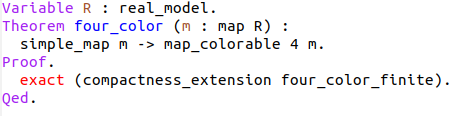
\includegraphics[height=2cm]{fourcolor.png}


\end{frame}


\subsection{}
\begin{frame}{Prouveurs automatiques}

Les prouveurs automatiques sont des logiciels formels
\begin{itemize}
    \item automatiques,
    \item à la logique plus restreinte,
    \item qui peuvent ne pas renvoyer de résultat,
    \item auxquels on accorde moins de confiance.
\end{itemize}

\hspace{1cm}

\texttt{(set-logic QF\_UF) \hfill ; logique utilisée}\\
\texttt{(declare-fun x () Bool) \hfill ; déclaration du booléen x}\\
\texttt{(assert (and x (not x)))\hfill ; hypothèse }\\
\texttt{(check-sat)}\\
\texttt{(exit)}
\end{frame}


\subsection{}
\begin{frame}{Certificats de veriT}

Si le problème n'est pas satisfiable, certains prouveurs automatiques renvoient un fichier de certificat qui explique pourquoi c'est le cas.

\hspace{1cm}

Dans le certificat de veriT suivant, le résultat de la dernière règle est la clause vide \texttt{()} qui représente l'absurde.

\begin{align*}
    1&:(input\,\,(x \wedge \neg x)) &\texttt{; hypothèse } x \wedge \neg x\\
    2&:(andproj \,\,(x) \,\,1\,\, 0) &\texttt{; de } x \wedge \neg x \texttt{, on obtient } x \\
    3&:(andproj \,\,(\neg x)\,\, 1\,\, 1) &\texttt{; de } x \wedge \neg x \texttt{, on obtient } \neg x\\
    4&:(resolution \,\,() \,\,3\,\, 2) &\texttt{; de } x \texttt{ et } \neg x \texttt{, on obtient } ()
\end{align*}

    
    
\end{frame}



\section{SMTCoq}

\subsection{}
\begin{frame}{Présentation de SMTCoq}
SMTCoq est une interface entre Coq et différents prouveurs automatiques qui est actuellement développée par Chantal Keller en collaboration avec l'Université de l'Iowa. \\
\vspace*{7mm}
But : amélioration de l'automatisation de Coq et de la confiance dans les prouveurs automatiques. \\
\vspace*{7mm}
Permet de prouver automatiquement le théorème suivant :
\[ \forall x \forall y \forall f. x \neq y + 1 \vee f(y) = f(x-1) \]
Fragment supporté : logique propositionnelle, arithmétique linéaire sur $\mathbb{Z}$, égalité et fonctions non-interprétées, variables quantifiées universellement en tête de formule.

\end{frame}

\subsection{}
\begin{frame}{Automatisation dans les assistants de preuve}
Deux approches à l'intégration d'un prouveur automatique dans un assistant de preuve :
\begin{multicols}{2}
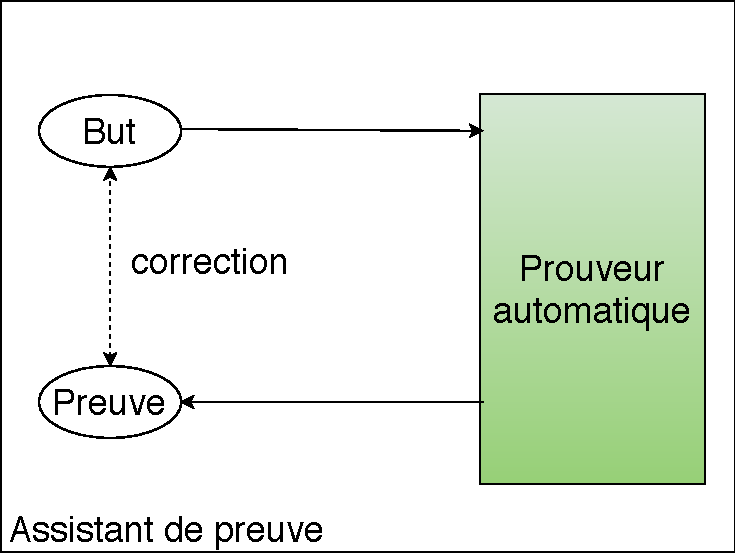
\includegraphics[height=4cm]{1_Autarcique.pdf}\\
Approche autarcique : vérifier le code du prouveur automatique.
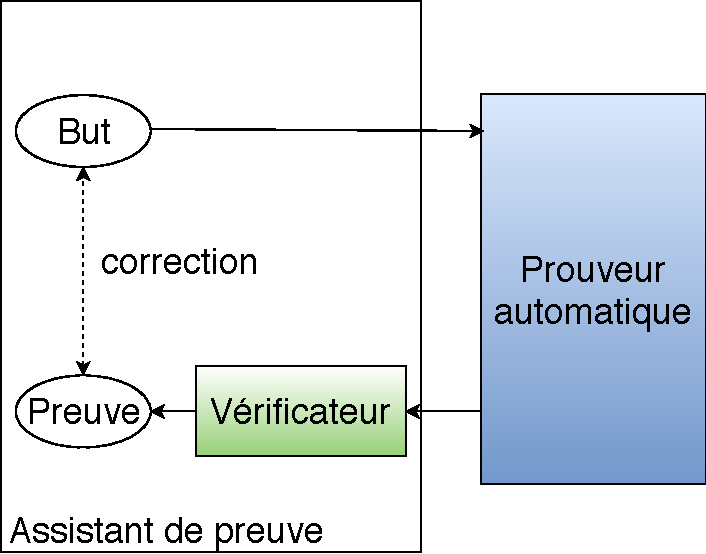
\includegraphics[height=4cm]{2_Sceptique.pdf}\\
Approche sceptique : vérifier la réponse du prouveur automati- que à chaque appel de celui-ci.
\end{multicols}
\end{frame}


\subsection{}
\begin{frame}{Approche sceptique}

\begin{center}
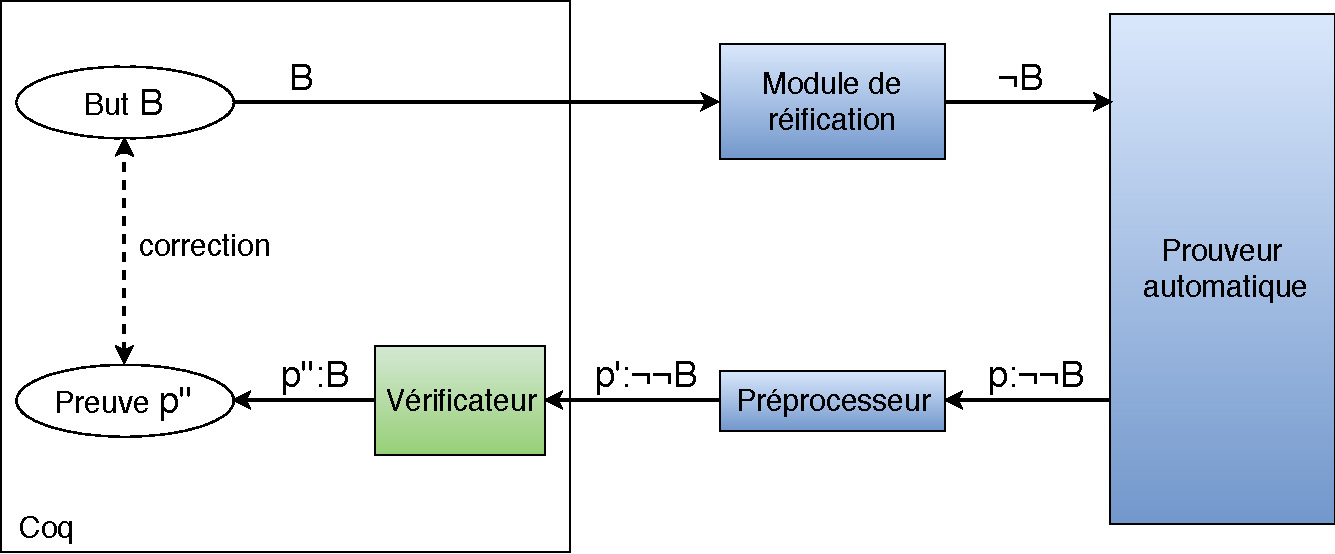
\includegraphics[height=4.4cm]{smtcoq_auto.pdf}
\end{center}

En transmettant la négation du but au prouveur automatique, on obtient un certificat prouvant l'absurde. Dans les cas d'application de SMTCoq, la double négation du but implique le but.


\end{frame}


\subsection{}
\begin{frame}{Réification}
    Réification : rendre explicite la structure d'un terme.
    
    \vspace{3mm}
    
    Par exemple, en notant \texttt{||} la fonction Coq qui implémente la disjonction booléenne, la structure du terme \[ \texttt{(true\,||\,false)\,||\,(false\,||\,true)}\]
    est donnée par l'arbre suivant :
    \begin{center}
    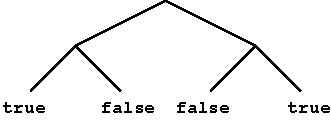
\includegraphics[height=2cm]{booltree.pdf}
    \end{center}
    Cet arbre peut être représenté dans une structure de données.
    
    \vspace{3mm}
    
    La structure du terme réifié est alors directement manipulable, on peut l'écrire dans un format adapté aux prouveurs automatiques.
\end{frame}

\subsection{}
\begin{frame}{Préprocesseur}
Le préprocesseur de SMTCoq remplit plusieurs objectifs :
\begin{itemize}
    \item \textbf{parsing} des fichiers de certificats en un type de données Ocaml
    \item \textbf{adaptations} des certificats, celles-ci sont par exemple nécessaires lorsque la logique du prouveur automatique diffère de celle de Coq
    \item \textbf{simplifications} en regroupant les règles du certificat au fonctionnement similaire
    \item \textbf{optimisations} des certificats, par exemple en élaguant les règles redondantes
\end{itemize}
\end{frame}

\subsection{}
\begin{frame}{Vérificateur : la fonction \textit{checker}}
On reprend le certificat de veriT donné en exemple : 
\begin{align*}
    & 1:(input\,\,(x \wedge \neg x))\\
    & \only<2->{2:(andproj \,\,(x) \,\,1\,\, 0)}\\
    & \only<3->{3:(andproj \,\,(\neg x)\,\, 1\,\, 1)}\\
    & \only<4->{4:(resolution \,\,() \,\,3\,\, 2)}
\end{align*}

En notant $inp := x \wedge \neg x$, l'état est initialisé à $[inp; inp; inp; inp]$.

\vspace{2mm}

\only<2->{La règle $2$ tranforme l'état en $[inp; x; inp; inp]$.}

\vspace{2mm}


\only<3->{La règle $3$ tranforme l'état en $[inp; x; \neg x; inp]$.}

\vspace{2mm}


\only<4->{La règle $4$ tranforme l'état en $[inp; x; \neg x; ()]$.}

\vspace{2mm}


\only<4->{Le résultat de \textit{checker} sur ce certificat et avec l'état initialisé comme ci-dessus est donc $true$.}
    
\end{frame}

\subsection{}
\begin{frame}{Vérificateur : le théorème de correction}

\begin{block}{ Théorème de correction}
Si \texttt{checker certif = true} où \texttt{certif} est un certificat ayant pour \texttt{input} la formule $f$ alors $f$ est fausse.
\end{block}

\textit{Point clé de la preuve} : le lemme de correction d'une étape.\\
Ce lemme nous assure que chaque règle modifie un emplacement de l'état en une formule vraie dans l'état courant.


\vspace{5mm}

Pour rétablir la preuve de correction lorsqu'on ajoute un nouveau type de règle, il suffit de compléter ce lemme pour ce nouveau type.
  
\vspace{5mm}

L'hypothèse du théorème de correction est obtenue en lançant le calcul de la fonction \textit{checker}, c'est la réflexion calculatoire.
  
  
\end{frame}





\section{Ajout de lemmes quantifiés}


\subsection{}
\begin{frame}{Amélioration de l'expressivité}
SMTCoq ne sait pas montrer que :
\[\forall h. homme(h) \Rightarrow mortel(h)\]
\[homme(Socrate)\]
implique :
\[mortel(Socrate)\]
\vspace*{2mm} \\
Objectifs du stage : permettre l'ajout de lemmes quantifiés au contexte et tenir compte de leurs instanciations dans le certificat.
\vspace*{6mm}\\
\end{frame}

\subsection{}
\begin{frame}{Ajout de lemmes au contexte}
\begin{center}
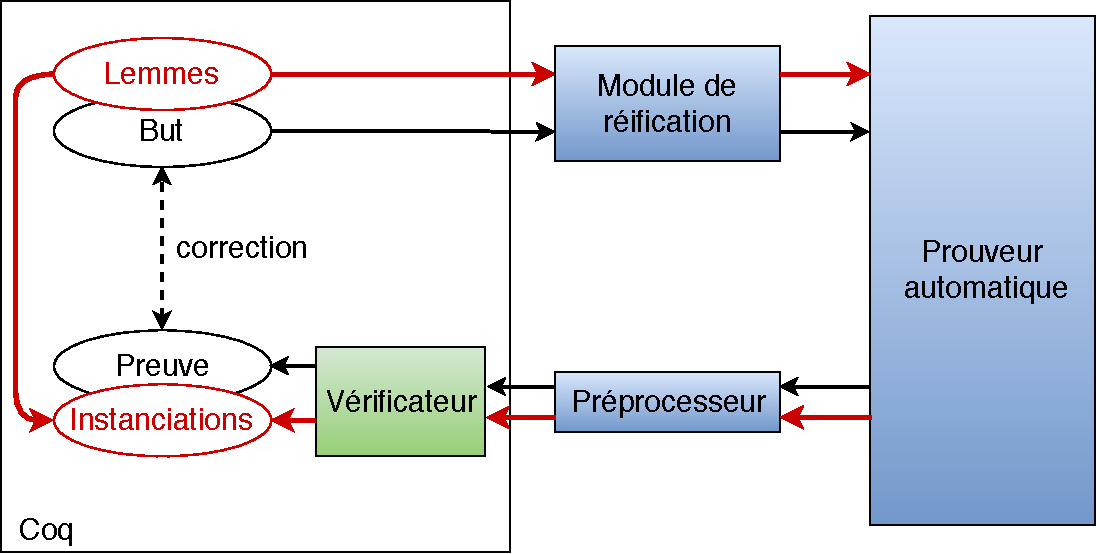
\includegraphics[height=5cm]{3_Contrib_Stage.pdf}
\end{center}
\end{frame}



\subsection{}
\begin{frame}{Règle \texttt{forall\_inst}}

La règle \texttt{forall\_inst} permet d'instancier les lemmes quantifiés donnés en \texttt{input} dans les certificats de veriT.

\vspace{1cm}

Forme générale des certificats avec règle \texttt{forall\_inst} : 
\begin{align*}
1&:(input \,\,(\forall x, P \,\, x))) &\texttt{; le lemme quantifié} \\
2&:(forall\_inst \,\,(\neg (\forall x, P \,\, x) \vee (P \, \, c) )) &\texttt{; instanciation du lemme} \\
3&:(resolution  \,\, (P \,\,c) \,\,1 \,\,2) & \text{; utilisation}
\end{align*}
    
\end{frame}

\subsection{}
\begin{frame}{Utilisation directe de la règle \texttt{forall\_inst}}
Une règle \texttt{forall\_inst} fait intervenir des formules de la forme :
\[  \neg (\forall x, P \,\, x) \vee (P \, \, c)  \]

L'utilisation directe de cette règle par le vérificateur pose plusieurs problèmes :

\begin{itemize}
\item logique classique vs logique intuitionniste
\item traitement des règle \texttt{input}
\item traitement des quantificateurs dans les règles
\end{itemize}
\end{frame}

\subsection{}
\begin{frame}{Modifications de la règle \texttt{forall\_inst}}

Le préprocesseur transforme la formule 
\[  \neg (\forall x, P \,\, x) \vee (P \, \, c)  \] 
en 
\[  P \, \, c \]

\vspace{5mm}

$\Longrightarrow$ Suppression de la forme logique de l'implication et des quantificateurs.
    
\vspace{5mm}    
    
Dans l'exemple, la règle \texttt{resolution} devient redondante.    
    
\end{frame}


\subsection{}
\begin{frame}{Autres difficultés rencontrées}

\textit{Parsing} : il faut reconnaître les quantificateurs. Problème des variables liées et \textit{hash consing}. 

\vspace{5mm}    
    
Reconnaître à quel lemme correspond une instance, veriT peut faire des modifications des instances.

\vspace{5mm}    

Montrer que le lemme reconnu implique l'instance, ici aussi les modifications de veriT posent problème.


\end{frame}


\subsection{}
\begin{frame}{Résultats du stage}

La commande \texttt{Add\_lemmas} ajoute les lemmes donnés en argument au contexte. Si aucun lemme n'est donné, la tactique \texttt{verit} garde le même fonctionnement que dans la version initiale de SMTCoq.

\vspace{3mm}
Un exemple en Coq :

\begin{center}
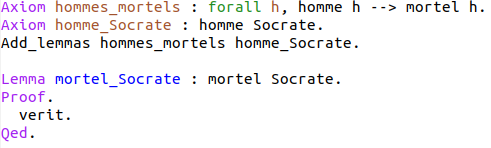
\includegraphics[height=2.5cm]{socrate.png}
\end{center}
\vspace{3mm}

$\longrightarrow $ \texttt{github.com/QGarchery/smtcoq-1}


\end{frame}



\end{document}

























